\documentclass[]{article}
\usepackage{lmodern}
\usepackage{amssymb,amsmath}
\usepackage{ifxetex,ifluatex}
\usepackage{fixltx2e} % provides \textsubscript
\ifnum 0\ifxetex 1\fi\ifluatex 1\fi=0 % if pdftex
  \usepackage[T1]{fontenc}
  \usepackage[utf8]{inputenc}
\else % if luatex or xelatex
  \ifxetex
    \usepackage{mathspec}
  \else
    \usepackage{fontspec}
  \fi
  \defaultfontfeatures{Ligatures=TeX,Scale=MatchLowercase}
\fi
% use upquote if available, for straight quotes in verbatim environments
\IfFileExists{upquote.sty}{\usepackage{upquote}}{}
% use microtype if available
\IfFileExists{microtype.sty}{%
\usepackage{microtype}
\UseMicrotypeSet[protrusion]{basicmath} % disable protrusion for tt fonts
}{}
\usepackage{hyperref}
\hypersetup{unicode=true,
            pdftitle={Epigenomic assessment of cardiovascular disease risk and interactions with traditional risk metrics},
            pdfborder={0 0 0},
            breaklinks=true}
\urlstyle{same}  % don't use monospace font for urls
\usepackage{graphicx,grffile}
\makeatletter
\def\maxwidth{\ifdim\Gin@nat@width>\linewidth\linewidth\else\Gin@nat@width\fi}
\def\maxheight{\ifdim\Gin@nat@height>\textheight\textheight\else\Gin@nat@height\fi}
\makeatother
% Scale images if necessary, so that they will not overflow the page
% margins by default, and it is still possible to overwrite the defaults
% using explicit options in \includegraphics[width, height, ...]{}
\setkeys{Gin}{width=\maxwidth,height=\maxheight,keepaspectratio}
\IfFileExists{parskip.sty}{%
\usepackage{parskip}
}{% else
\setlength{\parindent}{0pt}
\setlength{\parskip}{6pt plus 2pt minus 1pt}
}
\setlength{\emergencystretch}{3em}  % prevent overfull lines
\providecommand{\tightlist}{%
  \setlength{\itemsep}{0pt}\setlength{\parskip}{0pt}}
\setcounter{secnumdepth}{0}
% Redefines (sub)paragraphs to behave more like sections
\ifx\paragraph\undefined\else
\let\oldparagraph\paragraph
\renewcommand{\paragraph}[1]{\oldparagraph{#1}\mbox{}}
\fi
\ifx\subparagraph\undefined\else
\let\oldsubparagraph\subparagraph
\renewcommand{\subparagraph}[1]{\oldsubparagraph{#1}\mbox{}}
\fi

%%% Use protect on footnotes to avoid problems with footnotes in titles
\let\rmarkdownfootnote\footnote%
\def\footnote{\protect\rmarkdownfootnote}

%%% Change title format to be more compact
\usepackage{titling}

% Create subtitle command for use in maketitle
\providecommand{\subtitle}[1]{
  \posttitle{
    \begin{center}\large#1\end{center}
    }
}

\setlength{\droptitle}{-2em}

  \title{Epigenomic assessment of cardiovascular disease risk and interactions
with traditional risk metrics}
    \pretitle{\vspace{\droptitle}\centering\huge}
  \posttitle{\par}
    \author{}
    \preauthor{}\postauthor{}
    \date{}
    \predate{}\postdate{}
  
\usepackage{booktabs}
\usepackage{longtable}
\usepackage{array}
\usepackage{multirow}
\usepackage{wrapfig}
\usepackage{float}
\usepackage{colortbl}
\usepackage{pdflscape}
\usepackage{tabu}
\usepackage{threeparttable}
\usepackage{threeparttablex}
\usepackage[normalem]{ulem}
\usepackage{makecell}
\usepackage{xcolor}

\usepackage{booktabs}
\usepackage{longtable}
\usepackage{array}
\usepackage{multirow}
\usepackage{wrapfig}
\usepackage{float}
\usepackage{pdflscape}
\usepackage{tabu}
\usepackage{threeparttable}
\usepackage{threeparttablex}
\usepackage[normalem]{ulem}
\usepackage{makecell}

\begin{document}
\maketitle

\hypertarget{abstract}{%
\section{Abstract}\label{abstract}}

Background: Epigenome-wide association studies for cardiometabolic risk
factors have discovered multiple loci associated with incident
cardiovascular disease (CVD). However, few studies have sought to
directly optimize a predictor of CVD risk. Furthermore, it is
challenging to train multivariate models across multiple studies in the
presence of study- or batch effects.

Methods and Results: Here, we analyzed existing DNA methylation data
collected using the Illumina HumanMethylation450 microarray to create a
predictor of CVD risk across three cohorts: Women's Health Initiative,
Framingham Heart Study Offspring Cohort, and Lothian Birth Cohorts. We
trained Cox proportional hazards-based elastic net regressions for
incident CVD separately in each cohort, and used a recently-introduced
cross-study learning approach to integrate these individual scores into
an ensemble predictor. The methylation-based risk score (MRS) was
associated with CVD time-to-event in a held-out fraction of the
Framingham dataset (HR per SD=1.28, 95\% CI: 1.10-1.50) and predicted
myocardial infarction status in the independent REGICOR dataset (OR per
SD=2.14, 95\% CI: 1.58-2.89). These associations remained after
adjustment for traditional cardiovascular risk factors and were similar
to those from elastic net models trained on a directly merged dataset.
Additionally, we investigated interactions between the MRS and both
genetic and biochemical CVD risk, showing preliminary evidence of an
enhanced performance in those with less traditional risk factor
elevation.

Conclusions: This investigation provides proof-of-concept for a
genome-wide, CVD-specific epigenomic risk score and suggests that the
DNA methylation data may enable the discovery of high-risk individuals
that would be missed by alternative risk metrics.

Key Words: Epigenomics, DNA methylation, cardiovascular disease, risk
prediction

\hypertarget{introduction}{%
\section{Introduction}\label{introduction}}

DNA methylation is an important epigenetic pathway through which genetic
variants and environmental exposures impact disease
risk\textsuperscript{1,2}. Methylation at specific
cytosine-phosphate-guanine (CpG) sites has been associated with disease
in epigenome-wide association studies, even showing associations in
blood as a convenient but non-target tissue such as for type 2
diabetes\textsuperscript{3}. Methylation-based risk scores allow
genome-wide aggregation of epigenetic information, similarly to the more
established genetic risk scores, and allow for the use of models with
arbitrary complexity. These risk scores are often developed initially by
using methylation as a proxy for disease risk factors, such as body mass
index (BMI)\textsuperscript{4} and general aging-related
morbidity\textsuperscript{5}. Alternatively, given sufficient sample
size, epigenetic associations with disease risk can be modeled
directly\textsuperscript{6}.

Associations between DNA methylation and cardiovascular disease (CVD)
have been explored in many different cohorts and using diverse
approaches. Cross-sectional associations have been found across multiple
relevant tissues, namely blood, aorta, and other vascular
tissues\textsuperscript{7}. Some investigations aimed at cardiovascular
risk factors have discovered CpGs predictive of CVD
development\textsuperscript{8,9}, while Mendelian randomization
approaches have suggested causality of at least some of these CpG-risk
factor associations\textsuperscript{10}. A few studies directly modeling
incident CVD as a primary outcome have either been conducted using only
global (not locus-specific) methylation levels\textsuperscript{11}, or
have found limited additional predictive power in the presence of known
risk factors\textsuperscript{12}. A recent large-scale meta-analysis
found multiple CpG sites predictive of incident coronary heart disease,
but focused on univariate approaches\textsuperscript{13}. We have
previously investigated methylation regions and modules associating with
incident CVD, generating mechanistic insights but without aggregating
these results into a direct predictor of risk\textsuperscript{14}.
Additionally, it is unclear how the CVD risk tracked by DNA methylation
is redundant with or complementary to existing risk metrics, including
genetic scores\textsuperscript{15} and those based on traditional
cardiovascular risk factors (e.g.~the Framingham Risk Score for
generalized CVD)\textsuperscript{16}.

Combining signal across population-scale cohorts can increase sample
size while attenuating the effect of study-specific biases and
confounding factors, but can be prone to emergent sources of confounding
from ``batch'' effects or other systematic biases in methylation data
across cohorts. This is especially problematic when there is notable
class imbalance (i.e.~different outcome frequencies) across
cohorts\textsuperscript{17}. The most common method for dealing with
this heterogeneity is meta-analysis, but standard meta-analysis
approaches are restricted to univariate (one CpG site at a time) models.
Other approaches include batch effect correction on the input dataset
(e.g.~ComBat\textsuperscript{18}), direct adjustment for batch/study in
linear models, or adjustment for derived variables intended to capture
technical biases (e.g.~surrogate variable analysis\textsuperscript{19}),
but these approaches can often lead to over- or under-estimates of true
biological effects\textsuperscript{17}. An alternative approach
described recently, cross-study learning, instead trains an ensemble
predictor consisting of one or multiple models per
cohort\textsuperscript{20}. This strategy allows the use of arbitrarily
complex models while avoiding technical confounding from direct
combination of the datasets.

In order to develop an improved DNA methylation-based cardiovascular
risk predictor using multiple heterogeneous training cohorts, we used a
cross-study learning method to develop an ensemble of penalized
time-to-event regression risk models. The resulting composite risk score
performed well in a held-out data subset, associating with survival even
in the presence of traditional risk factors, and showing similar
performance to models trained on naively merged datasets. External
validation was achieved in a case-control study for prevalent myocardial
infarction (MI). Further, interactions were assessed between the
composite methylation-based risk score and other risk predictors,
finding that it is potentially most effective in those with low
Framingham Risk Scores.

\hypertarget{methods}{%
\section{Methods}\label{methods}}

\hypertarget{study-participants-and-phenotype-collection}{%
\subsection{Study participants and phenotype
collection}\label{study-participants-and-phenotype-collection}}

Phenotypes (demographic, anthropometric, biochemical, and clinical), DNA
methylation data, and imputed genotypes were available either from
publicly available controlled-access databases or upon request from the
cohorts. Cohort-specific details are provided in Supplementary methods.
Blood-based biochemical markers (total cholesterol, LDL-cholesterol,
HDL-cholesterol, triglycerides, fasting glucose, high-sensitivity
C-reactive protein, and systolic blood pressure) were log10-transformed
for all analyses. In the Lothian Birth Cohort 1936, LDL was estimated
from total cholesterol and triglycerides using the Friedewald equation.
Diabetes was defined as either use of diabetes medication or a measured
fasting blood glucose level of \textgreater{}125 mg/dL. Antihypertensive
medication use, smoking status, and diabetes status were assumed to be
false where missing, though missing data rates for these variables in
the held-out FHS subset were low (0.1\%, 0.1\%, and 7\%, respectively).
Analysis of these datasets was approved by the Tufts University Health
Sciences Institutional Review Board (protocol 12592), and all subjects
gave informed consent.

\hypertarget{dna-methylation-data-processing}{%
\subsection{DNA methylation data
processing}\label{dna-methylation-data-processing}}

DNA methylation data for all initial cohorts (WHI, FHS, and LBC) were
collected using the Illumina HumanMethylation450 microarray
platform\textsuperscript{21} and downloaded as raw intensity files. FHS
methylation data were collected in two primary batches in two centers --
one in subjects from a nested case-control for CVD measured at Johns
Hopkins University (FHS-JHU), and the other in a larger set of remaining
Framingham Offspring participants measured at the University of
Minnesota (FHS-UM). Preprocessing was performed using the \emph{minfi}
and \emph{wateRmelon} packages for R\textsuperscript{22,23}. Sample-wise
filters were as follows: robust overall signal in the main cluster based
on visual inspection of an intensity plot, less than 10\% of probes
undetected at a detection threshold of p\textless{}1e-16, and a reported
sex matching methylation-based sex prediction. Probes were removed using
the following criteria: more than 10\% of samples undetected at a
detection threshold of p\textless{}1e-16, location in the X or Y
chromosomes, non-CpG probes, cross-hybridizing probes, probes measuring
SNPs, and probes with an annotated SNP at the CpG site or in the
single-base extension region. Samples were normalized using the Noob
method for background correction and dye-bias normalization, followed by
the BMIQ method for probe type correction\textsuperscript{24,25}. Blood
cell fractions for 6 blood cell types (CD4+ T-cells, CD8+ T-cells,
B-cells, natural killer cells, monocytes, and granulocytes) were
estimated using a common reference-based method\textsuperscript{26}, and
5 of these (excluding granulocytes) were included in cell count-adjusted
statistical models. After quality control and filtering steps, 390597
CpG sites were shared between the 3 datasets, formatted as beta values
(roughly equal to the ratio of methylated signal to total microarray
signal, or \(\beta=\frac{M}{M+U+100}\)).

DNA methylation data for the REGICOR cohort were collected using the
Illumina MethylationEPIC microarray platform\textsuperscript{27} and
analyzed using the \emph{wateRmelon}\textsuperscript{23} and
methylumi\textsuperscript{28} R packages. Samples were excluded based on
detection p-value \textgreater{}0.05 in at least 1\% of probes or
failure to cluster in the appropriate sex based on X chromosome
methylation. Probes were excluded based on detection p-value
\textgreater{}0.05 in at least 1\% of samples, a bead count \textless{}3
in at least 5\% of samples, discarding by Illumina based on
underperformance (n=1,031) or changes in the manufacturing process
(n=977), non-CpG targets, and cross-hybridization (n=43,979). A batch
normalization was performed by standardizing beta values to mean zero
and unit variance within each bisulfite conversion batch prior to
analysis. After quality control and preprocessing, 811,610 CpG sites
across 391 individuals were available for analysis. Participants were
further excluded from analysis due to unknown smoking habits (n=10) and
unavailable information regarding diabetes, hypertension, or
hyperlipidemia (n=53). Surrogate variable analysis\textsuperscript{19}
was used to calculate two surrogate variables, representing potential
technical and biological confounders, for adjustment in MRS replication
models.

\hypertarget{cvd-risk-modeling}{%
\subsection{CVD risk modeling}\label{cvd-risk-modeling}}

Study-specific CVD risk models were trained using penalized Cox
proportional hazards regressions with the elastic net penalty. CVD
events were defined as including coronary heart disease, stroke, and
death from CVD (see Supplementary Methods for cohort-specific details),
and times were right-censored based on the most recent exam available in
each cohort. The elastic alpha parameter was initially set at 0.05
(closer to ridge regression) in order to retain a higher number of CpGs
with non-zero weights while still performing feature
selection\textsuperscript{29}. Inner cross-validation loops varying
alpha between 0.05 and 0.95 showed negligible differences in model
performance (evaluted by mean squared error). The penalty parameter
\(\lambda\) was optimized through 5-fold cross-validation (use of
10-fold cross-validation did not meaningfully change the results). For
each model, only the most variable 100,000 CpGs according to median
absolute deviation (\textasciitilde{}25\% of all available sites shared
across platforms) were included in order to decrease the computational
burden and ensure that the selected CpGs would have meaningful
interindividual variation.

The cross-study learner (CSL) was constructed as an ensemble of
study-specific regression models. Scores from each single-study learner
(SSL) were combined using the ``stacking'' approach\textsuperscript{20},
implemented as follows. First, predictions from each SSL to both itself
and the other training datasets were combined into a design matrix (with
dimensions \(N_{total}\) x \# SSLs). This formed the input to an
additional penalized Cox regression (ridge regression with \(\lambda\)
optimized through 5-fold CV and coefficients restricted to be
non-negative) of all training studies at once. Coefficients from this
regression, corresponding to input study-specific SSLs, were normalized
to sum to one to produce the CSL weights. For use in new datasets, SSL
scores were each standardized to mean zero and unit variance before
calculating their weighted sum (using the ``stacking'' weights) as the
final CSL score.

A series of approaches for combining information across cohorts were
tested as alternatives to the CSL. The naive ``combined'' approach
consisted of simply aggregating observations from all training sets into
a single dataset and training an elastic net regression as described
above while adjusting for study as a fixed effect. The ComBat method
trained across all studies as with the ``combined'' approach, but
included an empirical Bayes-based preprocessing step to directly remove
mean differences across studies that were not associated with the
outcome of interest (incident CVD events)\textsuperscript{18}.

MRS evaluation in FHS-UM was performed using Cox proportional hazards
models, with a series of models adjusting for covariates including
demographics, anthropometrics, biochemical values, and cell subtype
estimates. Additional sensitivity models incorporated flexible spline
bases for age and cell type fractions (\emph{pspline} function) and an
interaction between age and sex. Robust standard errors were used to
account for family structure as has been suggested for clustered
data\textsuperscript{30} and used for epigenetic risk models in
FHS\textsuperscript{31}. The proportional hazards assumption was
assessed using the \emph{cox.zph} R function, and no violation was
detected (p \textgreater{} 0.05). To compare risk scores generated using
different models (combined and ComBat-preprocessed) to the CSL, Cox
regressions adjusting for the ``basic'' covariate set were used to
evaluate each MRS alone, the CSL MRS plus the combined MRS, and the CSL
MRS plus the ComBat-preprocessed MRS in the held-out FHS-UM dataset.
Likelihood ratio tests were then used to compare each of the two-MRS
models to that CSL-only model, with the resulting p-values indicating
whether either of these alternative scores provided additional benefit.
MRS evaluation in the REGICOR case-control used logistic regression
models, adjusting for the same sets of covariates where possible, though
traditional biochemical risk factors were only available in discrete low
vs.~high categories.

The biology underlying the CSL model was evaluated through a series of
enrichment tests using the component CpG loci and annotated genes. Gene
ontology-based enrichment analysis of each cohort-specific model was
performed using the gometh function from the \emph{missMethyl} package
for R\textsuperscript{32}. This procedure uses gene annotations for CpGs
from the HumanMethylation450 microarray annotation from Illumina (v1.0
B2). Enrichment analysis is then performed for each gene ontology
category using Wallenius' noncentral hypergeometric distribution to
account for inconsistent representation of CpG sites across genes. The
overall merged set of CpGs included in the final CSL model was then
tested for enrichment in transcription factor binding sites using HOMER
tool\textsuperscript{33}. CpG loci (with respect to genome build hg19)
were provided as inputs, with 200 base-pair windows and repeat-masked
sequences.

\hypertarget{genomic-risk-score-calculation}{%
\subsection{Genomic risk score
calculation}\label{genomic-risk-score-calculation}}

Imputed genotype data for WHI were retrieved from dbGaP (accession:
phs000746.v2.p3. Variants were filtered for imputation R-squared
\textgreater{} 0.3, and annotated with rsIDs, loci, and allelic
information using the 1000 Genomes Phase 3 download from dbSNP (download
date: April 13, 2018). Weights for the genetic risk score calculation
(6,630,151 variants) were based on the genome-wide CVD score developed
by Khera et al\textsuperscript{15}. We note that these scores were
developed only for populations of European descent, and thus are not
optimized for the mixed-ancestry WHI population. GRS were then
calculated as the weighted sum of allelic dosages, normalized by the
number of relevant SNPs available. Genotype data processing and GRS
calculation were performed using PLINK 2.0.

\hypertarget{risk-score-interaction-analysis}{%
\subsection{Risk score interaction
analysis}\label{risk-score-interaction-analysis}}

Interaction analysis was performed using similar Cox regression models
to those above, adjusting for the ``basic'' set of covariates and using
robust standard error estimates. To facilitate visual comparisons,
main-effect regressions for the MRS were fitted within risk strata
defined by the FRS or GRS separately in each dataset. To obtain overall
interaction effect estimates, an interaction between MRS and either FRS
or GRS was introduced into a combined regression including all datasets,
while allowing stratified baseline hazards (strata() argument to the
coxph function). We note that main effects in the interaction analysis
are biased away from the null since the regression datasets were used
for training the MRS. Regressions assessing the GRS excluded non-white
participants to match the ancestry used to develop the CVD
score\textsuperscript{15}.

For quasi-replication of these associations in the REGICOR dataset,
stratified logistic regressions were used to discriminate MI cases from
controls using the MRS, while adjusting for estimated cell count
fractions as well as two SVA components (as in the main REGICOR models).
In the absence of continuous values for blood pressure and lipids, an
empirical risk function was generated by first performing a logistic
regression on the following cardiovascular risk factors: age, sex,
estimated cell count fractions, BMI, diabetes, smoking status,
hyperlipidemia (binary), and hypertension (binary), along with two SVA
components. Predicted risks based on this model were then used to
stratify subjects into four risk groups by evenly splitting the range of
predicted risks into four segments (thus resulting in strata based on
raw risk, rather than percentiles).

\hypertarget{results}{%
\section{Results}\label{results}}

\hypertarget{cross-study-learner-model-development}{%
\subsection{Cross-study learner model
development}\label{cross-study-learner-model-development}}

Epigenomic model development was performed in three cohorts, including
the Women's Health Initiative (WHI), Framingham Heart Study Offspring
Cohort (FHS), and Lothian Birth Cohort 1936 (LBC). The FHS dataset was
divided into two functionally separate groups (FHS-JHU and FHS-UM) based
on differences in subject selection and geographic location of
laboratory methylation analysis (see Methods). Further population
details can be found in Table 1.

\begin{table}

\caption{\label{tab:pop-description}Baseline parameters of the populations used for model development}
\centering
\begin{threeparttable}
\begin{tabular}[t]{lllll}
\toprule
Study/Subset & WHI & FHS-JHU & LBC & FHS-UM\\
Sample size & 2023 & 484 & 818 & 2103\\
Age & 65 (59-70) & 71 (64-77) & 69 (68-70) & 64 (59-71)\\
Sex (female) & 2023 (100\%) & 145 (30\%) & 406 (50\%) & 1270 (60\%)\\
\addlinespace[0em]
\multicolumn{5}{l}{Ancestry}\\
\hspace{1em}\% European & 959 (47\%) & 484 (100\%) & 818 (100\%) & 2103 (100\%)\\
\hspace{1em}\% African American & 651 (32\%) & 0 (0\%) & 0 (0\%) & 0 (0\%)\\
\hspace{1em}\% Hispanic & 413 (20\%) & 0 (0\%) & 0 (0\%) & 0 (0\%)\\
Body mass index (kg/m\textasciicircum{}2) & 29.1 (25.5-33.3) & 28.2 (25.5-31.3) & 27.5 (24.9-30.3) & 27.4 (24.3-31)\\
LDL cholesterol (mg/dL) & 150 (126-175) & 88 (73-107) & 118 (89.5-150.3) & 107 (87-128)\\
HDL cholesterol (mg/dL) & 51 (43-60) & 49 (40-60) & 56.1 (47.2-68.3) & 56 (45.8-69)\\
Triglycerides (mg/dL) & 127 (92-177) & 101.5 (75-141.2) & 128.4 (97.4-171.2) & 102 (73-142)\\
Fasting glucose (mg/dL) & 96 (88.6-108) & 106 (97-116) & Unavailable & 100 (94-109)\\
Systolic blood pressure (mm Hg) & 131 (120-143) & 130 (117-143) & 148.7 (137-161.3) & 126 (116-138)\\
\addlinespace[0em]
\multicolumn{5}{l}{\# CVD events}\\
\hspace{1em}Prior only & 0 & 127 & 70 & 112\\
\hspace{1em}Incident only & 1009 & 67 & 133 & 146\\
\hspace{1em}Prior and incident & 0 & 58 & 164 & 34\\
\hspace{1em}Total & 1009 & 252 & 367 & 292\\
Follow-up time (years) & 22 & 10 & 14 & 10\\
\bottomrule
\end{tabular}
\begin{tablenotes}
\item * Continuous values shown as: median (interquartile range)
\item WHI = Women's Health Initiative, FHS-JHU = Framingham Heart Study Offspring Cohort (Johns Hopkins University subset), LBC = Lothian Birth Cohorts 1936, FHS-UM = Framingham Heart Study Offspring Cohort (University of Minnesota subset)
\end{tablenotes}
\end{threeparttable}
\end{table}

Fig. 1 outlines the computational workflow. Briefly, a cross-study
learning (CSL) model was developed by training time-to-event elastic net
regressions on three of the datasets, while holding out the FHS-UM
subset for evaluation. The FHS-UM subset was chosen to hold out as it
more closely represents the larger free-living Framingham population.
While there is moderate heterogeneity between the included cohorts (for
example, in original cohort study designs, details of CVD definitions,
and length of follow-up), the intent of the present investigation was to
explore the extraction of shared signal across cohorts with recognized
heterogeneity. Next, a model re-trained on all four datasets was subject
to external replication in the REGICOR study. CSL model CpGs were
characterized as to their potential biological function, and model
performance was assessed across strata of alternative cardiovascular
risk metrics.

The initial predictor was developed by training individual penalized Cox
proportional hazards regression models (single-study learners, or SSLs)
in each of the three training cohorts (WHI, FHS-JHU, and LBC). Scores
from these models were aggregated through a ``stacking'' method, in
which the outcomes and model predictions from each of the individual
datasets are combined, and a regression is used to assign weights to
each of the model scores (see Methods). This procedure led to FHS-JHU
dropping out of the ensemble model, with weights for this initial
predictor as follows: 0.57 (WHI), 0.0 (FHS-JHU), and 0.43 (LBC). This
result means that the FHS-JHU score did not transfer to the rest of the
datasets (i.e.~to WHI and LBC) as well as the scores from the other two
components models.

\begin{figure}
\centering
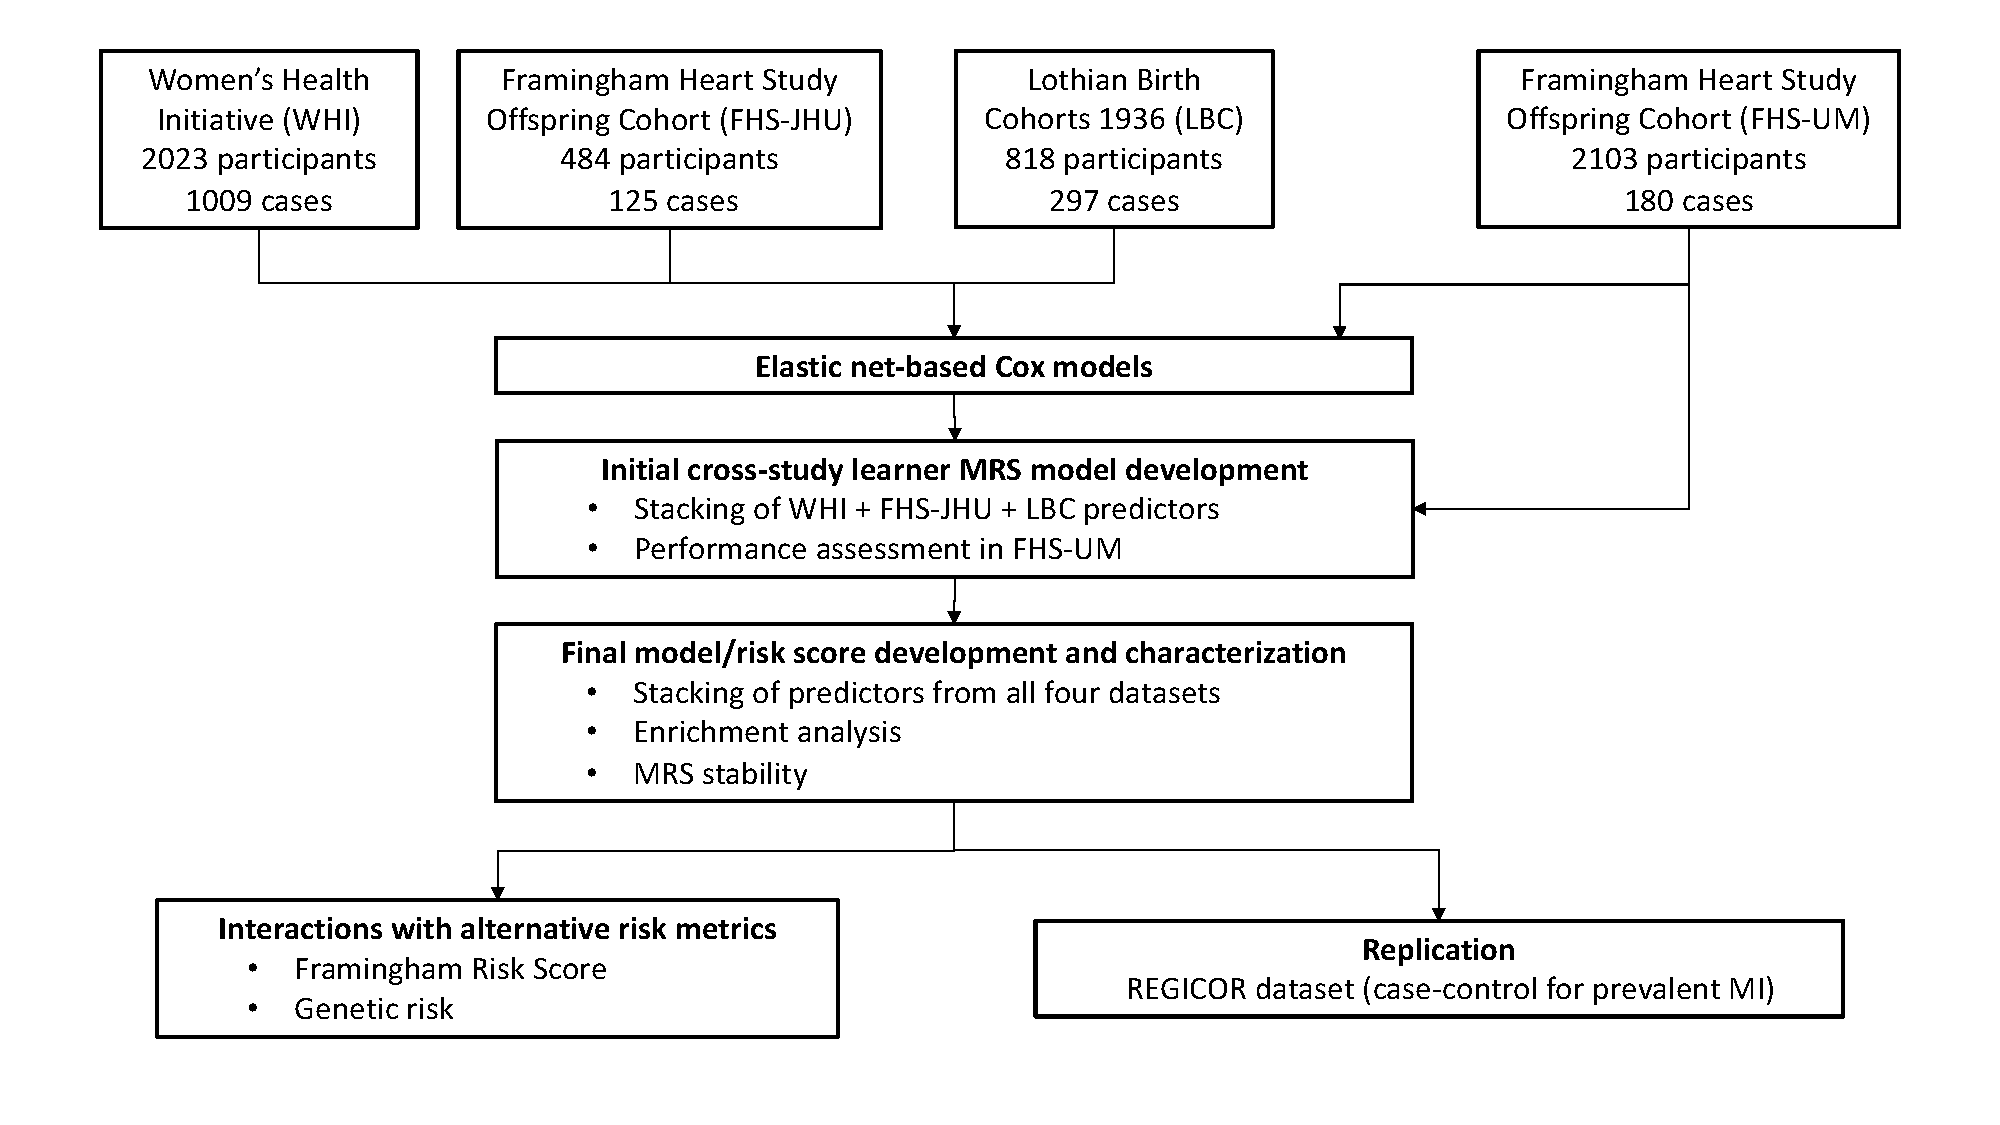
\includegraphics{workflow.pdf}
\caption{Computational workflow for MRS development and evaluation. The
initial MRS was trained in three cohorts with FHS-UM held out to
evaluate performance. The final MRS was then trained using all four
datasets and examined for biological significance, before testing for
prevalent MI discrimination in an independent cohort and assessment of
interactions with genetic and traditional risk scores.}
\end{figure}

\hypertarget{assessment-in-held-out-fhs-subset}{%
\subsection{Assessment in held-out FHS
subset}\label{assessment-in-held-out-fhs-subset}}

\begin{table}

\caption{\label{tab:fhs-holdout}MRS performance in held-out FHS subset}
\centering
\begin{threeparttable}
\begin{tabular}[t]{lll}
\toprule
Model & HR per s.d. MRS\textsuperscript{a} & P-value\\
\midrule
Unadjusted\textsuperscript{1} & 1.58 [1.37-1.83] & 5.4e-10\\
Basic\textsuperscript{2} & 1.28 [1.1-1.5] & 2.0e-03\\
Plus risk factors\textsuperscript{3} & 1.29 [1.09-1.51] & 2.7e-03\\
FRS only\textsuperscript{4} & 1.36 [1.19-1.58] & 2.0e-05\\
\bottomrule
\end{tabular}
\begin{tablenotes}
\item[a] Estimated hazard ratio per standard deviation of the methylation-based risk score
\item[1] No covariates
\item[2] Adjusted for age, sex, and estimated cell type fractions
\item[3] Additionally adjusted for BMI, LDL, HDL, SBP, diabetes status, and current smoking
\item[4] Adjusted for Framingham Risk Score only (uses all risk factors other than BMI and cell type fractions)
\end{tablenotes}
\end{threeparttable}
\end{table}

\begin{verbatim}
## Setting levels: control = FALSE, case = TRUE
\end{verbatim}

\begin{verbatim}
## Setting direction: controls < cases
\end{verbatim}

\begin{verbatim}
## Setting levels: control = FALSE, case = TRUE
\end{verbatim}

\begin{verbatim}
## Setting direction: controls < cases
\end{verbatim}

\begin{verbatim}
## Setting levels: control = FALSE, case = TRUE
\end{verbatim}

\begin{verbatim}
## Setting direction: controls < cases
\end{verbatim}

\begin{figure}
\centering
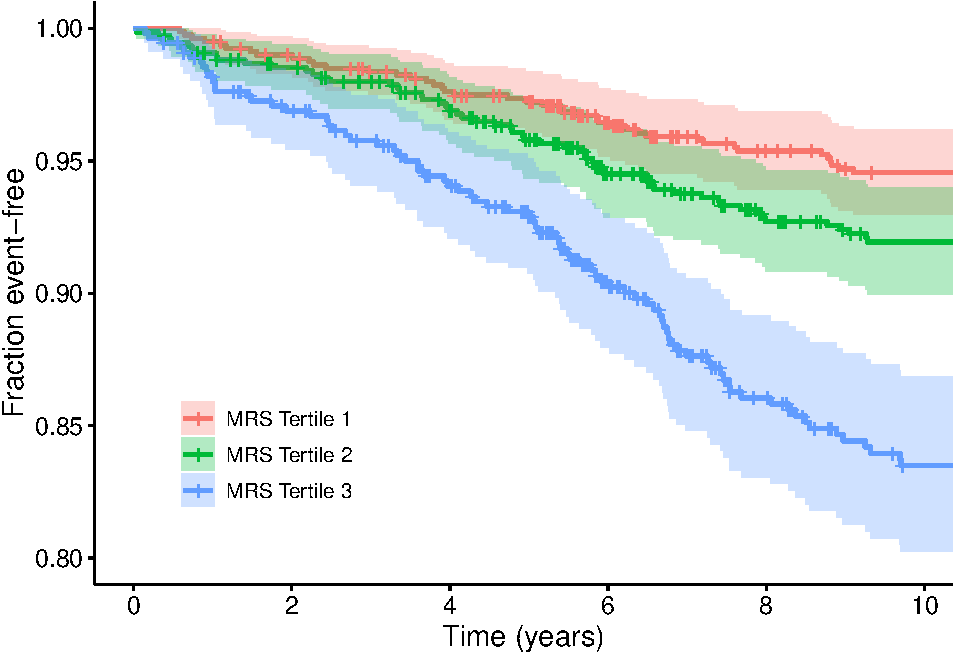
\includegraphics{figures/km-plot-1.pdf}
\caption{Kaplan-Meier survival curves in the held-out FHS-UM dataset.
Individual curves correspond to tertiles of the initial (3-dataset) MRS.
Vertical ticks correspond to censored observations, and colored bands
represent 95\% confidence intervals for tertile-specific survival
curves. X-axis is limited to the time span in which at least 50
uncensored observations remained for each tertile (3275 days).}
\end{figure}

Stacking of the three initial predictors resulted in model weights of
0.57, 0, and 0.43 for WHI, FHS-JHU, and LBC, respectively (i.e.~the
FHS-JHU sub-model did not contribute to the initial stacked ensemble
model). The resulting ensemble predictor was evaluated using robust Cox
proportional hazards models in FHS-UM, showing strong associations with
incident CVD in an unadjusted model (HR=1.58, 95\% CI: 1.37-1.83), which
was attenuated partially through adjustment for standard covariates
(age, sex, and estimated cell type fractions; HR=1.28, 95\% CI:
1.10-1.50) as well as CVD risk factors (HR=1.29, 95\% CI: 1.09-1.51).
Results for the unadjusted model and three risk factor-adjusted models
are shown in Table 2, and associated Kaplan-Meier curves across
epigenetic risk tertiles are shown in Fig. 2.

Additional sensitivity analyses were performed to assess the robustness
of these results to variations in the model-building or evaluation
approach. Hazard ratios in the held-out FHS-UM were no higher using
penalized logistic regression in training (unadjusted HR=1.52, 95\% CI:
1.32-1.76), excluding individuals with past events in training
(unadjusted HR=1.55, 95\% CI: 1.33-1.81), or adjusting for race in WHI
(unadjusted HR=1.20, 95\% CI: 1.03-1.39). Neither were these results
affected by training using the full set of 390,597 CpGs. Similarly,
variations in the evaluation regressions did not produce meaningfully
different results, either when excluding all individuals who experienced
prior CVD events (Supp. Table S1), analyzing incident CVD as a binary
outcome using logistic regression (unadjusted odds ratio per standard
deviation=2.15, 95\% CI: 1.91-2.42), or stratifying by sex. Adjustment
for age and cell type fractions as flexible spline functions as well as
an age-sex interaction to assess possible residual confounding did not
decrease estimated HRs from the Basic model (saturated model HR=1.31,
95\% CI: 1.12-1.52). Use of the MRS for binary incident CVD prediction
resulted in a c-statistic of 0.642 (95\% CI: 0.599-0.685), compared to
0.691 (95\% CI: 0.653-0.729) for the Framingham Risk Score alone and
0.695 (95\% CI: 0.655-0.734) using the two scores together.

Results from comparison of CSL performance to models trained on combined
datasets (either naive combination or including preprocessing using
ComBat) are shown in Supp. Fig. S1. The ComBat-preprocessed model had
modestly higher hazard ratios in FHS-UM, while relative differences with
the combined model depended on the covariates included. However,
likelihood ratio tests using the Basic model covariates (age, sex, and
cell type fraction-adjusted) did not reveal a strong added benefit of
either the combined (p = 0.58) or ComBat (p = 0.08) risk scores over
that using only the CSL.

\hypertarget{final-csl-model-characterization}{%
\subsection{Final CSL model
characterization}\label{final-csl-model-characterization}}

\begin{figure}
\centering
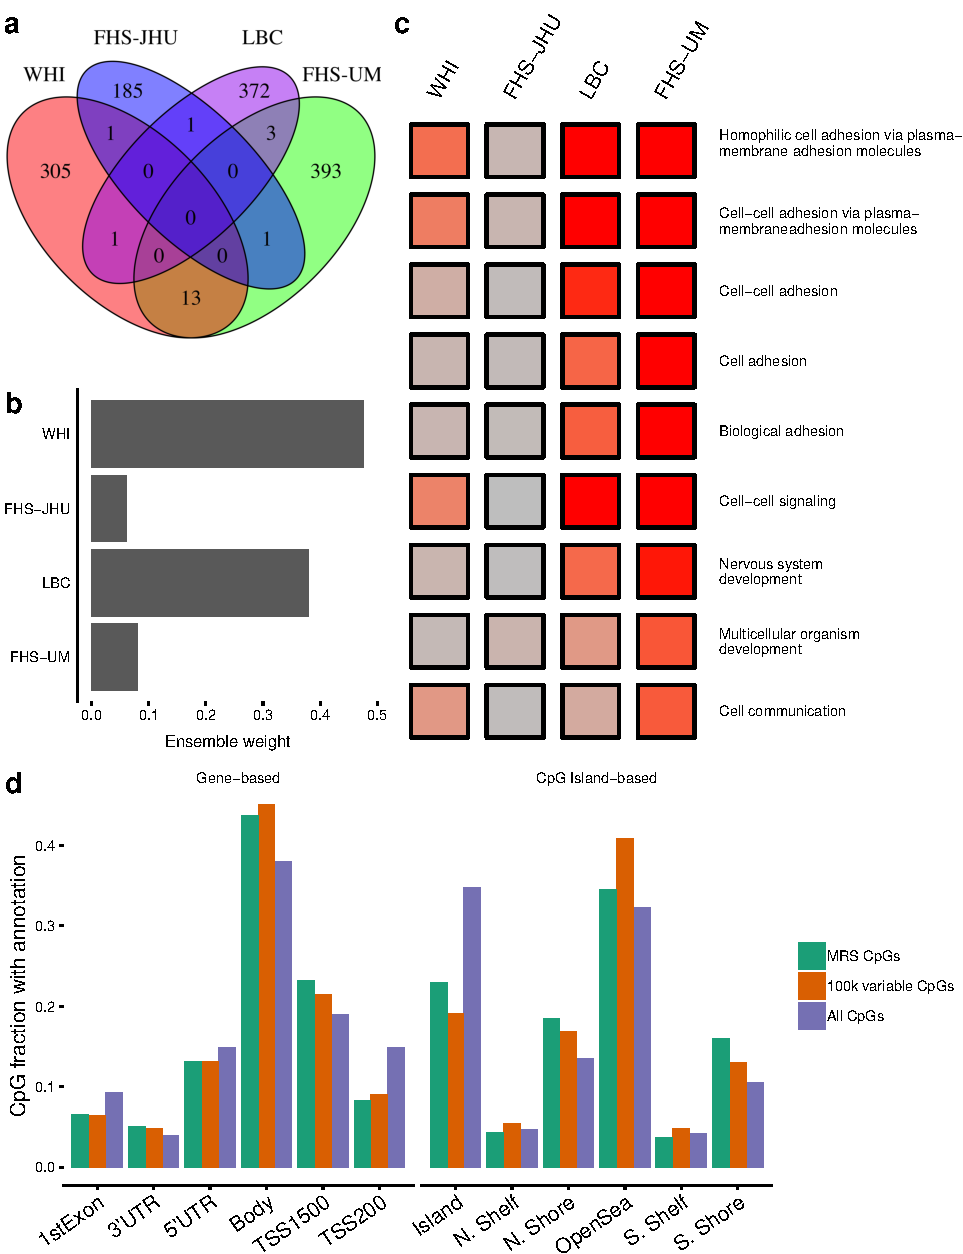
\includegraphics{figures/characterization-1.pdf}
\caption{Characterization of the final CSL model. a) Overlap of CpG
sites in the four individual predictors constituting the final model. b)
Study-specific weights for constructing the ensemble model (derived from
the ``stacking'' regression). c) Results from Gene Ontology-based
enrichment analysis using genes annotated to SSL component CpGs. All GO
terms with false discovery rate \textless{} 0.001 in any cohort are
shown, and colored according to -log(p-value) for enrichment in each
SSL. Values were cut at -log(p) = 20 for visualization purposes. d)
Proportion of CpGs in the full set of CSL CpGs (union of CpG sets in
each component SSL) compared to the 100,000 most variable CpGs (as used
in SSL model development) and the full set of available CpGs. Groupings
according to both gene-based and CpG island-based CpG annotations are
shown.}
\end{figure}

The stacking regression in the final CSL model defining the
methylation-based risk score (MRS) gave the most weight to WHI (0.48)
and LBC (0.38), while retaining nonzero weights for FHS-JHU (0.06) and
FHS-UM (0.08). This result indicates that the WHI and LBC-trained models
were better able to transfer across the combined-cohort set of outcomes
compared to the other models. There was little overlap of specific CpG
sites across cohort-specific models, with a maximum of 13 CpGs shared
between two models (WHI and FHS-UM) and no CpGs shared between three or
more models (Fig. 3a). This could result from heterogeneity in the
complex relationships between DNA methylation and CVD across
populations. However, it may also reflect the tendency of the elastic
net regression to select only a single feature from a group of
correlated features, where the specific CpGs selected in different
datasets varied due to the presence of biological and technical noise.
However, even if the SSLs were capturing different biological
mechanisms, the CSL model is designed to capture such heterogeneous
signal from across cohorts. Despite the lack of site-specific overlap,
there was broad agreement for three of the four component SSL models at
the level of enriched biological processes, with all except FHS-JHU
enriched most strongly for proximity to genes involved in homophilic
cell adhesion (Fig. 3b). MRS component CpGs tended to be found in
similar genomic loci to the overall set of variable CpGs, and were
enriched in gene bodies and depleted in CpG islands compared to the full
microarray CpG set. However, MRS CpGs did show a modest enrichment in
and around CpG islands compared to the set of variable CpGs (Fig. 3d).
To seek more clarity as to potential biological mechanisms represented
by the MRS, the HOMER tool was used to calculate enrichment of
transcription factor (TF) binding motifs in the MRS component CpG sites.
Using the union of all individual SSL CpG sites as input, no strong
enrichments were found (all q-values \textgreater{}0.5).

To better understand the stability of the risk score over time,
intraclass correlation coefficients (ICCs) were calculated for two sets
of grouped samples: 26 technical replicates from FHS and approximately
1000 longitudinal samples (across 3 visits, or about 6 years total) from
LBC (Supp. Table S2). The technical replicates showed an ICC of 0.85,
while the longitudinal samples showed an ICC of 0.68. As would be
expected, the ICC for samples closer in time (Waves 1 \& 2; ICC = 0.69)
were higher than that for samples more distant in time (Waves 1 \& 3;
ICC = 0.61). Based on the observation of imperfect stability of the MRS
over time as well as the partial attenuation in held-out hazard ratios
after adjustment for age, its component CpGs (the 1305-element union of
all CpGs in any of the four individual SSL models) were examined for
overlap with established epigenetic age metrics. While no enrichment was
seen for the original cross-tissue DNAm age from
Horvath\textsuperscript{34}, strong enrichment was seen for the
morbidity-directed PhenoAge\textsuperscript{5} (9 of 513 CpGs; p=2.3e-5)
and especially the blood-specific aging marker from Hannum et
al.\textsuperscript{35} (13 of 71 CpGs; p=5.9e-21). We note that these
overlaps do not constitute a major fraction of either CpG set, but are
nonetheless highly statistically significant. The PhenoAge metric is
based on some known cardiovascular risk factors (e.g.~C-reactive
protein) and is known to associate with CVD, but is not trained in any
of the cohorts included here.

\hypertarget{discrimination-in-myocardial-infarction-case-control-study}{%
\subsection{Discrimination in myocardial infarction case-control
study}\label{discrimination-in-myocardial-infarction-case-control-study}}

\begin{table}

\caption{\label{tab:regicor}Results from replication in REGICOR MI case-control}
\centering
\begin{threeparttable}
\begin{tabular}[t]{llll}
\toprule
Model & ComBat & Combined & CSL\\
\midrule
Unadjusted & 1.79 [1.39-2.31] & 1.86 [1.45-2.38] & 1.83 [1.41-2.37]\\
Basic & 2.16 [1.58-2.93] & 2.12 [1.57-2.87] & 2.14 [1.58-2.89]\\
Plus risk factors & 1.76 [1.22-2.54] & 1.66 [1.15-2.4] & 1.61 [1.11-2.34]\\
\bottomrule
\end{tabular}
\begin{tablenotes}
\item * Results are presented as: OR per s.d. MRS [95\% CI]
\item * Model covariates as in Table 2
\item * All models above are adjusted for two surrogate variable analysis (SVA) components.
\end{tablenotes}
\end{threeparttable}
\end{table}

As one form of replication, the MRS was investigated for its
discriminative performance in a nested case-control for prior myocardial
infarction in the REGICOR cohort (Table 3; cohort description in Supp.
Table S3), which was matched for sex and age and thus free of potential
confounding by these variables. We note that this dataset contained
prevalent (rather than incident) events, and thus provides replication
in a similar but not identical biological context. These methylation
data were collected on the next generation of Illumina methylation
microarray (MethylationEPIC), which does not perfectly overlap with the
HumanMethylation450 platform, but contained approximately 93\% of the
CpGs input to the MRS model training procedure. The MRS was able to
discriminate cases and controls in both unadjusted (odds ratio = 1.79, p
= 6.33e-6) and, to a lesser degree, risk factor-adjusted models (odds
ratio = 1.61, p = 0.019). Odds ratios were qualitatively similar across
modeling strategies (Combined, ComBat, and CSL) for all of the
adjustment models (Supp. Fig. S1b).

\hypertarget{interactions-with-alternate-risk-metrics}{%
\subsection{Interactions with alternate risk
metrics}\label{interactions-with-alternate-risk-metrics}}

\begin{figure}
\centering
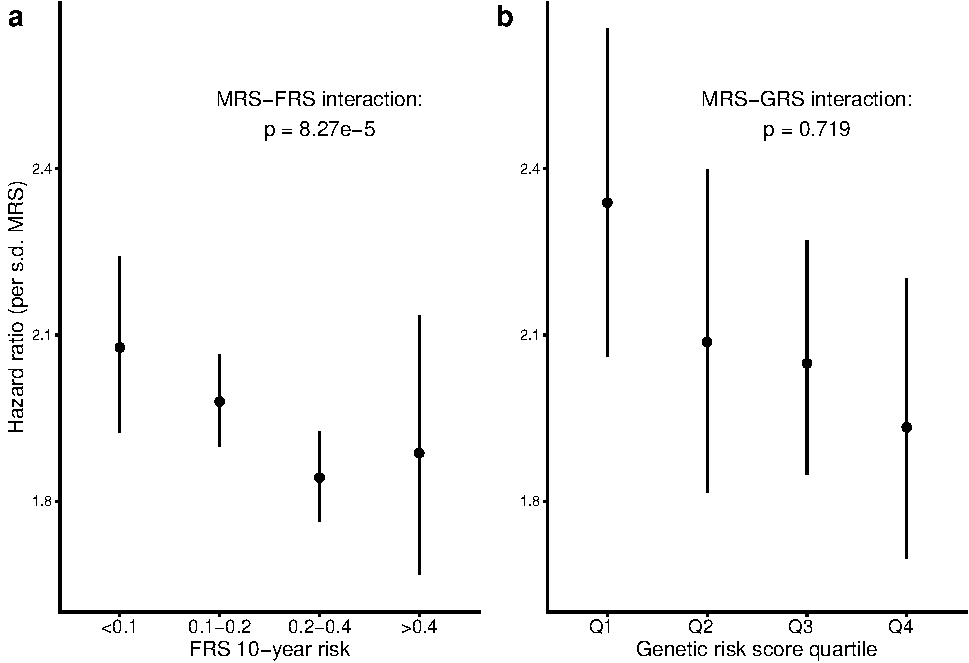
\includegraphics{figures/aggregate-interactions-1.pdf}
\caption{Interactions of MRS with other biomarkers of CVD risk. a)
Hazard ratios for the MRS within subsets of 10-year generalized CVD risk
according to the Framingham Risk Score. b) Hazard ratios for the MRS
within quartiles of a genetic cardiovascular risk score (in white WHI
participants only). Hazard ratios are estimated using the final MRS,
which was trained using each of these datasets. Cox regressions included
stratum-specific baseline hazards and were adjusted for age, sex, and
estimated cell subtype fractions. Error bars represent standard errors
for the hazard ratio estimates. Annotated p-values describe the test of
interaction between the MRS and the alternative risk metric.}
\end{figure}

To understand how the present risk score interacts with other
established CVD risk metrics, the performance of the MRS was
re-evaluated after stratifying individuals by risk scores reflecting
either demographic and biochemical features (Framingham Risk Score), or
genetic variants (based on Khera et al.~2018). First, the marginal
effects of these risk scores were confirmed in each population. The
Framingham Risk Score (FRS) was strongly predictive in WHI and FHS,
while surprisingly showing no association with CVD incidence in LBC
(Supp. Table S4). As the dataset with the largest number of available
events, the genetic score was evaluated in WHI, demonstrating a moderate
association with CVD (odds ratio per standard deviation = 1.28, p =
1.1e-6).

In pooled Cox models using study-specific baseline hazards and performed
using the final four-study MRS, it appeared that the MRS was more
effective in those in lower ``traditional'' risk strata (based on models
stratified by FRS categories; Fig. 4a). As a sensitivity analysis, the
cohorts were fully stratified into separate models, in which this
pattern was visually clear in WHI and FHS-JHU (Supp. Fig. S2). The
pattern did not appear in LBC, although we note that the Framingham Risk
Score also did not show a ``main effect'' for incident CVD in this
cohort. A similar pattern appeared with respect to genetic risk in WHI
(European ancestry participants only based on the formulation of the
relevant risk score), in which maximum MRS performance was achieved in
the lowest alternative risk stratum. Supplementing these visual
comparisons, combined Cox regressions across all cohorts (allowing for
different baseline hazards across studies) showed a strong MRS-FRS
interaction effect (7\% reduction in HR for the MRS per 10\% increase in
FRS; p = 8.27e-05), while that for the MRS-GRS interaction did not reach
nominal statistical significance (2\% reduction in HR for the MRS per
standard deviation increase in GRS; p = 0.719).

To explore the clinical potential of these interactions further, we
returned to the initial MRS (trained in 3 datasets with FHS-UM held
out). The FHS-UM dataset was filtered to include only participants with
lower CVD risk based on the FRS (\textless{}10\% estimated 10-year
risk). Within this lower-risk subset, participants in the upper MRS
quintile had more than double the risk of the remainder of the
participants: 7\% (12/176) of the upper MRS quintile experienced
incident events, while 3\% (19/701) of the remaining four MRS quintiles
experienced incident events.

FRS could not be calculated in the REGICOR dataset, as not all risk
factors were available as continuous values. However, stratified models
replicated the observation of greater MRS discrimination in the lowest
alternative risk stratum. An empirical risk function was generated
through logistic regression of MI status on cardiovascular risk factors
(age, sex, BMI, diabetes, smoking status, hyperlipidemia (binary), and
hypertension). Predicted MI risk using this model was used to stratify
subjects into four risk groups, with MRS odds ratios (per standard
deviation) of 4.49 in the lowest-risk group versus 1.20 in the
highest-risk group. More detailed results from these analyses are shown
in Supp. Table S5.

\hypertarget{discussion}{%
\section{Discussion}\label{discussion}}

Epigenetic signatures of cardiometabolic diseases and aging in general
are being actively explored as biomarkers of disease risk that are
potentially modifiable and reveal underlying biological mechanisms.
Here, in a novel application of a cross-study ensembling method, we
introduce a DNA methylation-based score specific to cardiovascular
disease risk. The model performs similarly to one trained on a direct
combination of the component datasets, and may perform best in
individuals predicted to be at lower risk based on traditional risk
factors.

We opted to use cross-study learning to train our risk model based on
the expectation that differences across cohorts (e.g.~demographic,
behavioral) may contribute to heterogeneity in both the marginal
distribution of the CpG features and the conditional distribution of the
CVD outcome. Under these conditions, the generalizability of a
single-study predictor is often obscured or
overstated\textsuperscript{36,37}. The performance of the CSL model was
similar to that of models trained on the merged cohorts with or without
batch adjustment via ComBat. This suggests that the assumptions made by
these direct combination strategies (i.e.~that the heterogeneity
structure can be captured by variation in the marginal effects of each
CpG site) are met. In practice, this underlying structure is unknown,
and we highlight that the CSL was able to produce similar gains in
accuracy without making specific assumptions.

In assessing the stability of the MRS, we observed reasonable
reproducibility between technical replicates (ICC=0.85). ICCs for LBC
subjects over time were somewhat lower (ICC=0.68), which is to be
expected due to not only changes in environment, but also the known
epigenetic evolution with age that we observed to be enriched in the
components of our score. Furthermore, this value is at the upper end of
the range of single-CpG repeatability measurements over time calculated
in the combined Lothian Birth Cohorts (1921 and
1936)\textsuperscript{38}. These ICC values suggest an imperfect but
usable reproducibility of the MRS, and an aggregate marker that is
fairly robust considering the low replicability that has been observed
for individual sites in technical replicates (general median ICC of 0.3
and mode of 0.75 in a ``high reliability'' cluster)\textsuperscript{39}.

Our observation that different CpGs tended to be selected across studies
(Fig. 3) is in agreement with the relative lack of replication seen in
prior cardiovascular epigenomic studies\textsuperscript{7}. However, the
enrichment of the MRS component CpGs for proximity to genes related to
cell-cell adhesion (in all subsets except FHS-JHU) is indicative of
shared underlying biological mechanisms. As we have previously observed
in the WHI and FHS cohorts, it appears that immune activation is central
to the prognostic information contained in leukocyte DNA
methylation\textsuperscript{{\textbf{???}}}. For example, epigenetic
processes have been shown to be involved in the activation and increased
adhesion of monocytes in response to environmental insults and metabolic
stress, though these have been explored primarily in relation to histone
modifications\textsuperscript{40}. Our results provide preliminary
support for an attractive model in which a methylation-based score could
act as a monitor of cumulative stress in leukocytes and their
corresponding activation towards a more atherogenic state.

Existing epigenetic scores have shown varying strengths of association
with incident cardiovascular disease. An early investigation examined
blood-based methylation in LINE-1 elements, finding strong associations
of global hypomethylation with prevalent and incident ischemic heart
disease (LINE-1), though additional reports showed opposite associations
of methylation at repetitive elements with CVD\textsuperscript{41}.
Guarrera et al.~developed a biomarker for MI based on global LINE-1 and
ZBTB12 gene methylation that provided a modest net reclassification
index improvement (0.23-0.47) compared to traditional risk factors only.
Multiple epigenetic aging metrics, though not developed specifically for
CVD, have been shown to predict incident CHD, including PhenoAge (odds
ratios from 1.02 to 1.08) and GrimAge (hazard ratio = 1.07, adjusted for
age and technical factors)\textsuperscript{5,31}. While these
associations are statistically significant, they do not represent
clinically meaningful improvements in discrimination. Our observed
hazard ratio of 1.28 (Basic model in the held-out FHS-UM dataset)
indicates that this MRS may be closer to clinical relevance. We note
that our component CpG sites overlap strongly with those of these
established epigenetic metrics including PhenoAge, suggesting that it
captures some of the same biological patterns. However, the mechanistic
significance of the specific methylation signals captured by these
aging-related metrics, whether as markers of epigenetic regulation
breakdown or the work of an ``epigenetic maintenance system'', is still
unclear\textsuperscript{34,42}.

In examining the potential clinical utility of an novel risk score for
CVD, it is important to understand to what extent it is redundant with
or complementary to existing risk metrics. We first note that the
strength of this epigenetic score in adjusted models is lower than that
found for traditional risk scores (Supp. Table S4) and some novel
biochemical risk measures such as high-sensitivity Troponin I (adjusted
HR for global CVD = 3.01)\textsuperscript{43}. However, analysis of
interactions between different risk metrics can be clinically relevant,
as demonstrated for example in a recent investigation exploring the
interaction between genetic and lifestyle-based risk prediction for
dementia\textsuperscript{44}. Here, we saw a pattern of stronger
epigenetic risk associations in individuals whose cardiovascular risk
based on traditional metrics (here, the Framingham Risk Score) was low.
This pattern replicated in the REGICOR dataset (though FRS could not be
directly calculated), with improved MRS discrimination in lower-risk
subjects based on an empirical risk function. While these associations
are preliminary, they suggest that an epigenetic risk score could help
identify higher-risk individuals who otherwise would not have been
detected by other metrics. While we did not identify any robust patterns
of differential MRS performance in strata based on a genetic
cardiovascular risk score, there may have been lower power to detect any
such patterns from the outset given the modest discriminatory
performance of the GRS in WHI.

Multiple limitations should be acknowledged. While lymphocytes are known
to be important in CVD pathogenesis, epigenetic signals have been
reported in other CVD-relevant tissues, such as aorta and other vascular
tissues\textsuperscript{7}, that were not examined here. Additionally,
the present definition of CVD was chosen to balance specificity of CVD
subtypes with sample size, but this balance could be altered to focus on
more specific disease subtypes (e.g.~myocardial infarction) or a broader
definition of CVD (e.g.~including heart failure). Finally, while the
REGICOR dataset provided an important age- and sex-matched case-control
setting for replication of the MRS, this work would benefit from future
replication in an independent cohort enabling assessment of incident
disease.

In sum, we have developed an epigenetic risk score for cardiovascular
disease that provides additional value beyond existing risk measures,
and may show improved performance in populations otherwise designated as
low-risk. Furthermore, we have shown a novel application of a
cross-cohort ensembling method that may provide significant value to
future investigations in genomic epidemiology.

\hypertarget{acknowledgements}{%
\section{Acknowledgements}\label{acknowledgements}}

We thank all LBC1936 study participants and research team members. The
LBC1936 is supported by Age UK (Disconnected Mind program) and the
Medical Research Council (MR/M01311/1). Methylation typing in LBC1936
was supported by Centre for Cognitive Ageing and Cognitive Epidemiology
(Pilot Fund award), Age UK, The Wellcome Trust Institutional Strategic
Support Fund, The University of Edinburgh, and The University of
Queensland. LBC1936 work was conducted in the Centre for Cognitive
Ageing and Cognitive Epidemiology, which is supported by the Medical
Research Council and Biotechnology and Biological Sciences Research
Council (MR/K026992/1), and which supported IJD.

\hypertarget{reproducibility}{%
\section{Reproducibility}\label{reproducibility}}

Code supporting the analyses described here can be found at
\url{https://github.com/kwesterman/meth_cvd}. Code and instructions
related to the original cross-study learning approach can be found at
\url{https://github.com/prpatil/csml_rep}.

\hypertarget{funding-sources}{%
\section{Funding Sources}\label{funding-sources}}

KW was supported by NIH predoctoral training grant 5T32HL069772-14.

\hypertarget{disclosures}{%
\section{Disclosures}\label{disclosures}}

None

\hypertarget{references}{%
\section*{References}\label{references}}
\addcontentsline{toc}{section}{References}

\hypertarget{refs}{}
\leavevmode\hypertarget{ref-Bonder2016}{}%
1. Bonder MJ, Luijk R, Zhernakova DV, Moed M, Deelen P, Vermaat M,
Iterson M van, Dijk F van, Galen M van, Bot J, Slieker RC, Jhamai PM,
Verbiest M, Suchiman HED, Verkerk M, Breggen R van der, Rooij J van,
Lakenberg N, Arindrarto W, Kielbasa SM, Jonkers I, van 't Hof P, Nooren
I, Beekman M, Deelen J, Heemst D van, Zhernakova A, Tigchelaar EF,
Swertz MA, Hofman A, Uitterlinden AG, Pool R, Dongen J van, Hottenga JJ,
Stehouwer CDA, Kallen CJH van der, Schalkwijk CG, Berg LH van den, Zwet
EW van, Mei H, Li Y, Lemire M, Hudson TJ, Slagboom PE, Wijmenga C,
Veldink JH, Greevenbroek MMJ van, Duijn CM van, Boomsma DI, Isaacs A,
Jansen R, Meurs JBJ van, 't Hoen PAC, Franke L, Heijmans BT. Disease
variants alter transcription factor levels and methylation of their
binding sites. \emph{Nature Genetics}. 2016;49:131--138.

\leavevmode\hypertarget{ref-Tobi2018}{}%
2. Tobi EW, Slieker RC, Luijk R, Dekkers KF, Stein AD, Xu KM, Slagboom
PE, Zwet EW van, Lumey LH, Heijmans BT. DNA methylation as a mediator of
the association between prenatal adversity and risk factors for
metabolic disease in adulthood. \emph{Science Advances}.
2018;4:eaao4364.

\leavevmode\hypertarget{ref-Bacos2016}{}%
3. Bacos K, Gillberg L, Volkov P, Olsson AH, Hansen T, Pedersen O,
Gjesing AP, Eiberg H, Tuomi T, Almgren P, Groop L, Eliasson L, Vaag A,
Dayeh T, Ling C. Blood-based biomarkers of age-associated epigenetic
changes in human islets associate with insulin secretion and diabetes.
\emph{Nature Communications}. 2016;7:11089.

\leavevmode\hypertarget{ref-Wahl2017}{}%
4. Wahl S, Drong A, Lehne B, Loh M, Scott WR, Kunze S, Tsai P-C, Ried
JS, Zhang W, Yang Y, Tan S, Fiorito G, Franke L, Guarrera S, Kasela S,
Kriebel J, Richmond RC, Adamo M, Afzal U, Ala-Korpela M, Albetti B,
Ammerpohl O, Apperley JF, Beekman M, Bertazzi PA, Black SL, Blancher C,
Bonder M-J, Brosch M, Carstensen-Kirberg M, Craen AJM de, Lusignan S de,
Dehghan A, Elkalaawy M, Fischer K, Franco OH, Gaunt TR, Hampe J, Hashemi
M, Isaacs A, Jenkinson A, Jha S, Kato N, Krogh V, Laffan M, Meisinger C,
Meitinger T, Mok ZY, Motta V, Ng HK, Nikolakopoulou Z, Nteliopoulos G,
Panico S, Pervjakova N, Prokisch H, Rathmann W, Roden M, Rota F, Rozario
MA, Sandling JK, Schafmayer C, Schramm K, Siebert R, Slagboom PE,
Soininen P, Stolk L, Strauch K, Tai E-S, Tarantini L, Thorand B,
Tigchelaar EF, Tumino R, Uitterlinden AG, Duijn C van, Meurs JBJ van,
Vineis P, Wickremasinghe AR, Wijmenga C, Yang T-P, Yuan W, Zhernakova A,
Batterham RL, Smith GD, Deloukas P, Heijmans BT, Herder C, Hofman A,
Lindgren CM, Milani L, Harst P van der, Peters A, Illig T, Relton CL,
Waldenberger M, Järvelin M-R, Bollati V, Soong R, Spector TD, Scott J,
McCarthy MI, Elliott P, Bell JT, Matullo G, Gieger C, Kooner JS,
Grallert H, Chambers JC. Epigenome-wide association study of body mass
index and the adverse outcomes of adiposity. \emph{Nature}.
2017;541:81--86.

\leavevmode\hypertarget{ref-Levine2018}{}%
5. Levine ME, Lu AT, Quach A, Chen BH, Assimes TL, Bandinelli S, Hou L,
Baccarelli AA, Stewart JD, Li Y, Whitsel EA, Wilson JG, Reiner AP, Aviv
A, Lohman K, Liu Y, Ferrucci L, Horvath S. An epigenetic biomarker of
aging for lifespan and healthspan. \emph{Aging}. 2018;10:573--591.

\leavevmode\hypertarget{ref-Hao2017}{}%
6. Hao X, Luo H, Krawczyk M, Wei W, Wang W, Wang J, Flagg K, Hou J,
Zhang H, Yi S, Jafari M, Lin D, Chung C, Caughey BA, Li G, Dhar D, Shi
W, Zheng L, Hou R, Zhu J, Zhao L, Fu X, Zhang E, Zhang C, Zhu J-K, Karin
M, Xu R-H, Zhang K. DNA methylation markers for diagnosis and prognosis
of common cancers. \emph{Proceedings of the National Academy of
Sciences}. 2017;114:7414--7419.

\leavevmode\hypertarget{ref-Fernandez-Sanles2017}{}%
7. Fernández-Sanlés A, Sayols-Baixeras S, Subirana I, Degano IR, Elosua
R. Association between DNA methylation and coronary heart disease or
other atherosclerotic events: A systematic review. 2017;263:325--333.

\leavevmode\hypertarget{ref-Hedman2017}{}%
8. Hedman ÅK, Mendelson MM, Marioni RE, Gustafsson S, Joehanes R, Irvin
MR, Zhi D, Sandling JK, Yao C, Liu C, Liang L, Huan T, McRae AF,
Demissie S, Shah S, Starr JM, Cupples LA, Deloukas P, Spector TD,
Sundström J, Krauss RM, Arnett DK, Deary IJ, Lind L, Levy D, Ingelsson
E. Epigenetic Patterns in Blood Associated With Lipid Traits Predict
Incident Coronary Heart Disease Events and Are Enriched for Results From
Genome-Wide Association Studies. \emph{Circulation: Cardiovascular
Genetics}. 2017;10:e001487.

\leavevmode\hypertarget{ref-Aslibekyan2018}{}%
9. Aslibekyan S, Agha G, Colicino E, Do AN, Lahti J, Ligthart S, Marioni
RE, Marzi C, Mendelson MM, Tanaka T, Wielscher M, Absher DM, Ferrucci L,
Franco OH, Gieger C, Grallert H, Hernandez D, Huan T, Iurato S, Joehanes
R, Just AC, Kunze S, Lin H, Liu C, Meigs JB, Meurs JBJ van, Moore AZ,
Peters A, Prokisch H, Räikkönen K, Rathmann W, Roden M, Schramm K,
Schwartz JD, Starr JM, Uitterlinden AG, Vokonas P, Waldenberger M, Yao
C, Zhi D, Baccarelli AA, Bandinelli S, Deary IJ, Dehghan A, Eriksson J,
Herder C, Jarvelin M-R, Levy D, Arnett DK. Association of Methylation
Signals With Incident Coronary Heart Disease in an Epigenome-Wide
Assessment of Circulating Tumor Necrosis Factor \(\alpha\). \emph{JAMA
Cardiology}. 2018;3:463--472.

\leavevmode\hypertarget{ref-Richardson2017}{}%
10. Richardson TG, Zheng J, Davey Smith G, Timpson NJ, Gaunt TR, Relton
CL, Hemani G. Mendelian Randomization Analysis Identifies CpG Sites as
Putative Mediators for Genetic Influences on Cardiovascular Disease
Risk. \emph{American Journal of Human Genetics}. 2017;101:590--602.

\leavevmode\hypertarget{ref-Baccarelli2010}{}%
11. Baccarelli A, Wright R, Bollati V, Litonjua A, Zanobetti A,
Tarantini L, Sparrow D, Vokonas P, Schwartz J. Ischemic heart disease
and stroke in relation to blood DNA methylation. \emph{Epidemiology}.
2010;21:819--828.

\leavevmode\hypertarget{ref-Guarrera2015}{}%
12. Guarrera S, Fiorito G, Onland-Moret NC, Russo A, Agnoli C, Allione
A, Di Gaetano C, Mattiello A, Ricceri F, Chiodini P, Polidoro S, Frasca
G, Verschuren MWM, Boer JMA, Iacoviello L, Schouw YT van der, Tumino R,
Vineis P, Krogh V, Panico S, Sacerdote C, Matullo G. Gene-specific DNA
methylation profiles and LINE-1 hypomethylation are associated with
myocardial infarction risk. \emph{Clinical Epigenetics}. 2015;7:133.

\leavevmode\hypertarget{ref-Agha2019}{}%
13. Agha G, Mendelson MM, Ward-Caviness CK, Joehanes R, Huan T, Gondalia
R, Salfati E, Brody JA, Fiorito G, Bressler J, Chen BH, Ligthart S,
Guarrera S, Colicino E, Just AC, Wahl S, Gieger C, Vandiver AR, Tanaka
T, Hernandez DG, Pilling LC, Singleton AB, Sacerdote C, Krogh V, Panico
S, Tumino R, Li Y, Zhang G, Stewart JD, Floyd JS, Wiggins KL, Rotter JI,
Multhaup M, Bakulski K, Horvath S, Tsao PS, Absher DM, Vokonas P,
Hirschhorn J, Fallin MD, Liu C, Bandinelli S, Boerwinkle E, Dehghan A,
Schwartz JD, Psaty BM, Feinberg AP, Hou L, Ferrucci L, Sotoodehnia N,
Matullo G, Peters A, Fornage M, Assimes TL, Whitsel EA, Levy D,
Baccarelli AA. Blood Leukocyte DNA Methylation Predicts Risk of Future
Myocardial Infarction and Coronary Heart Disease. \emph{Circulation}.
2019;140:645--657.

\leavevmode\hypertarget{ref-Westerman2019}{}%
14. Westerman K, Sebastiani P, Jacques P, Liu S, DeMeo D, Ordovás JM.
DNA methylation modules associate with incident cardiovascular disease
and cumulative risk factor exposure. \emph{Clinical Epigenetics}.
2019;11:142.

\leavevmode\hypertarget{ref-Khera2018}{}%
15. Khera AV, Chaffin M, Aragam KG, Haas ME, Roselli C, Choi SH,
Natarajan P, Lander ES, Lubitz SA, Ellinor PT, Kathiresan S. Genome-wide
polygenic scores for common diseases identify individuals with risk
equivalent to monogenic mutations. \emph{Nature Genetics}.
2018;50:1219--1224.

\leavevmode\hypertarget{ref-DAgostino2008}{}%
16. D'Agostino RB, Vasan RS, Pencina MJ, Wolf PA, Cobain M, Massaro JM,
Kannel WB. General cardiovascular risk profile for use in primary care:
The Framingham heart study. \emph{Circulation}. 2008;117:743--753.

\leavevmode\hypertarget{ref-Goh2017}{}%
17. Goh WWB, Wang W, Wong L. Why Batch Effects Matter in Omics Data, and
How to Avoid Them. 2017;35:498--507.

\leavevmode\hypertarget{ref-Johnson2007}{}%
18. Johnson WE, Li C, Rabinovic A. Adjusting batch effects in microarray
expression data using empirical Bayes methods. \emph{Biostatistics}.
2007;8:118--127.

\leavevmode\hypertarget{ref-Leek2007}{}%
19. Leek JT, Storey JD. Capturing Heterogeneity in Gene Expression
Studies by Surrogate Variable Analysis. \emph{PLoS Genetics}.
2007;3:e161.

\leavevmode\hypertarget{ref-Patil2018}{}%
20. Patil P, Parmigiani G. Training replicable predictors in multiple
studies. \emph{Proceedings of the National Academy of Sciences}.
2018;115:2578--2583.

\leavevmode\hypertarget{ref-Bibikova2011}{}%
21. Bibikova M, Barnes B, Tsan C, Ho V, Klotzle B, Le JM, Delano D,
Zhang L, Schroth GP, Gunderson KL, Fan J-B, Shen R. High density DNA
methylation array with single CpG site resolution. \emph{Genomics}.
2011;98:288--295.

\leavevmode\hypertarget{ref-Aryee2014}{}%
22. Aryee MJ, Jaffe AE, Corrada-Bravo H, Ladd-Acosta C, Feinberg AP,
Hansen KD, Irizarry RA. Minfi: A flexible and comprehensive Bioconductor
package for the analysis of Infinium DNA methylation microarrays.
\emph{Bioinformatics}. 2014;30:1363--1369.

\leavevmode\hypertarget{ref-Pidsley2013}{}%
23. Pidsley R, Y Wong CC, Volta M, Lunnon K, Mill J, Schalkwyk LC. A
data-driven approach to preprocessing Illumina 450K methylation array
data. \emph{BMC Genomics}. 2013;14:293.

\leavevmode\hypertarget{ref-Fortin2016}{}%
24. Fortin J-P, Triche TJ, Hansen KD. Preprocessing, normalization and
integration of the Illumina HumanMethylationEPIC array with minfi.
\emph{Bioinformatics}. 2016;33:btw691.

\leavevmode\hypertarget{ref-Teschendorff2013}{}%
25. Teschendorff AE, Marabita F, Lechner M, Bartlett T, Tegner J,
Gomez-Cabrero D, Beck S. A beta-mixture quantile normalization method
for correcting probe design bias in Illumina Infinium 450 k DNA
methylation data. \emph{Bioinformatics}. 2013;29:189--196.

\leavevmode\hypertarget{ref-Houseman2012}{}%
26. Houseman EA, Accomando WP, Koestler DC, Christensen BC, Marsit CJ,
Nelson HH, Wiencke JK, Kelsey KT. DNA methylation arrays as surrogate
measures of cell mixture distribution. \emph{BMC Bioinformatics}.
2012;13:86.

\leavevmode\hypertarget{ref-Pidsley2016}{}%
27. Pidsley R, Zotenko E, Peters TJ, Lawrence MG, Risbridger GP, Molloy
P, Van Djik S, Muhlhausler B, Stirzaker C, Clark SJ, Jones P, Baylin S,
Ko Y, Mohtat D, Suzuki M, Park A, Izquierdo M, Han S, Dayeh T, Volkov P,
Salo S, Hall E, Nilsson E, Olsson A, Pidsley R, Viana J, Hannon E,
Spiers H, Troakes C, Al-Saraj S, Stirzaker C, Taberlay P, Statham A,
Clark S, Clark S, Harrison J, Paul C, Frommer M, Lister R, Pelizzola M,
Dowen R, Hawkins R, Hon G, Tonti-Filippini J, Bibikova M, Le J, Barnes
B, Saedinia-Melnyk S, Zhou L, Shen R, Hinoue T, Weisenberger D, Lange C,
Shen H, Byun H, Berg D, Breitling L, Yang R, Korn B, Burwinkel B,
Brenner H, Rakyan V, Down T, Maslau S, Andrew T, Yang T, Beyan H,
Bibikova M, Barnes B, Tsan C, Ho V, Klotzle B, Le J, Morris T, Beck S,
Chen Y, Choufani S, Grafodatskaya D, Butcher D, Ferreira J, Weksberg R,
Chen Y, Lemire M, Choufani S, Butcher D, Grafodatskaya D, Zanke B, Naeem
H, Wong N, Chatterton Z, Hong M, Pedersen J, Corcoran N, Peters T,
Buckley M, Statham A, Pidsley R, Samaras K, Lord RV, Wang D, Yan L, Hu
Q, Sucheston L, Higgins M, Ambrosone C, Warden C, Lee H, Tompkins J, Li
X, Wang C, Riggs A, Lizio M, Harshbarger J, Shimoji H, Severin J,
Kasukawa T, Sahin S, Siggens L, Ekwall K, Dedeurwaerder S, Defrance M,
Calonne E, Denis H, Sotiriou C, Fuks F, Pidsley R, CC YW, Volta M,
Lunnon K, Mill J, Schalkwyk L, Teschendorff A, Marabita F, Lechner M,
Bartlett T, Tegner J, Gomez-Cabrero D, Touleimat N, Tost J, Thurman R,
Rynes E, Humbert R, Vierstra J, Maurano M, Haugen E, Andersson R,
Gebhard C, Miguel-Escalada I, Hoof I, Bornholdt J, Boyd M, Kundaje A,
Meuleman W, Ernst J, Bilenky M, Yen A, Ritchie M, Phipson B, Wu D, Hu Y,
Law C, Shi W, Stadler M, Murr R, Burger L, Ivanek R, Lienert F, Schöler
A, Ziller M, Gu H, Müller F, Donaghey J, Tsai L-Y, Kohlbacher O, Huang
S, Bao B, Hour T, Huang C, Yu C, Liu C, Neuhausen S, Slattery M, Garner
C, Ding Y, Hoffman M, Brothman A, Reams R, Kalari K, Wang H, Odedina F,
Soliman K, Yates C, Song J, Stirzaker C, Harrison J, Melki J, Clark S,
Coolen M, Stirzaker C, Song J, Statham A, Kassir Z, Moreno C, Makrides
M, Gibson R, McPhee A, Yelland L, Quinlivan J, Ryan P, Lawrence M,
Taylor R, Toivanen R, Pedersen J, Norden S, Pook D, Clark S, Statham A,
Stirzaker C, Molloy P, Frommer M, Auton A, Brooks L, Durbin R, Garrison
E, Kang H, Kent W. Critical evaluation of the Illumina MethylationEPIC
BeadChip microarray for whole-genome DNA methylation profiling.
\emph{Genome Biology}. 2016;17:208.

\leavevmode\hypertarget{ref-Davis2019}{}%
28. Davis S, Du P, Bilke S, Triche T, Bootwalla O. methylumi: Handle
Illumina methylation data. 2019.
doi:\href{https://doi.org/10.1016/j.neuroimage.2007.06.039}{10.1016/j.neuroimage.2007.06.039}.

\leavevmode\hypertarget{ref-Benton2017}{}%
29. Benton MC, Sutherland HG, Macartney-Coxson D, Haupt LM, Lea RA,
Griffiths LR. Methylome-wide association study of whole blood DNA in the
Norfolk Island isolate identifies robust loci associated with age.
\emph{Aging}. 2017;9:753--768.

\leavevmode\hypertarget{ref-Rogers1993}{}%
30. Rogers WH. Regression standard errors in clustered samples.
\emph{Stata Technical Bulletin}. 1993;13:19--23.

\leavevmode\hypertarget{ref-Lu2019}{}%
31. Lu AT, Quach A, Wilson JG, Reiner AP, Aviv A, Raj K, Hou L,
Baccarelli AA, Li Y, Stewart JD, Whitsel EA, Assimes TL, Ferrucci L,
Horvath S. DNA methylation GrimAge strongly predicts lifespan and
healthspan. \emph{Aging}. 2019;11:303--327.

\leavevmode\hypertarget{ref-Phipson2015}{}%
32. Phipson B, Maksimovic J, Oshlack A. MissMethyl: An R package for
analyzing data from Illumina's HumanMethylation450 platform.
\emph{Bioinformatics}. 2015;32:286--288.

\leavevmode\hypertarget{ref-Heinz2010}{}%
33. Heinz S, Benner C, Spann N, Bertolino E, Lin YC, Laslo P, Cheng JX,
Murre C, Singh H, Glass CK. Simple Combinations of Lineage-Determining
Transcription Factors Prime cis-Regulatory Elements Required for
Macrophage and B Cell Identities. \emph{Molecular Cell}.
2010;38:576--589.

\leavevmode\hypertarget{ref-Horvath2013}{}%
34. Horvath S. DNA methylation age of human tissues and cell types.
\emph{Genome biology}. 2013;14:R115.

\leavevmode\hypertarget{ref-Hannum2013}{}%
35. Hannum G, Guinney J, Zhao L, Zhang L, Hughes G, Sadda S, Klotzle B,
Bibikova M, Fan JB, Gao Y, Deconde R, Chen M, Rajapakse I, Friend S,
Ideker T, Zhang K. Genome-wide Methylation Profiles Reveal Quantitative
Views of Human Aging Rates. \emph{Molecular Cell}. 2013;49:359--367.

\leavevmode\hypertarget{ref-Chang2015}{}%
36. Chang CC, Chow CC, Tellier LC, Vattikuti S, Purcell SM, Lee JJ.
Second-generation PLINK: rising to the challenge of larger and richer
datasets. \emph{GigaScience}. 2015;4:7.

\leavevmode\hypertarget{ref-Zhang2018}{}%
37. Zhang Y, Bernau C, Parmigiani G, Waldron L. The impact of different
sources of heterogeneity on loss of accuracy from genomic prediction
models. \emph{Biostatistics}. 2018.
doi:\href{https://doi.org/10.1093/biostatistics/kxy044}{10.1093/biostatistics/kxy044}.

\leavevmode\hypertarget{ref-Shah2014}{}%
38. Shah S, McRae AF, Marioni RE, Harris SE, Gibson J, Henders AK,
Redmond P, Cox SR, Pattie A, Corley J, Murphy L, Martin NG, Montgomery
GW, Starr JM, Wray NR, Deary IJ, Visscher PM. Genetic and environmental
exposures constrain epigenetic drift over the human life course.
\emph{Genome Research}. 2014;24:1725--1733.

\leavevmode\hypertarget{ref-Bose2014}{}%
39. Bose M, Wu C, Pankow JS, Demerath EW, Bressler J, Fornage M, Grove
ML, Mosley TH, Hicks C, North K, Kao W, Zhang Y, Boerwinkle E, Guan W.
Evaluation of microarray-based DNA methylation measurement using
technical replicates: the Atherosclerosis Risk In Communities (ARIC)
Study. \emph{BMC Bioinformatics}. 2014;15:312.

\leavevmode\hypertarget{ref-Short2017}{}%
40. Short JD, Tavakoli S, Nguyen HN, Carrera A, Farnen C, Cox LA, Asmis
R. Dyslipidemic Diet-Induced Monocyte ``Priming'' and Dysfunction in
Non-Human Primates Is Triggered by Elevated Plasma Cholesterol and
Accompanied by Altered Histone Acetylation. \emph{Frontiers in
Immunology}. 2017;8:958.

\leavevmode\hypertarget{ref-Kim2010}{}%
41. Kim M, Long TI, Arakawa K, Wang R, Yu MC, Laird PW. DNA Methylation
as a Biomarker for Cardiovascular Disease Risk. \emph{PLoS ONE}.
2010;5:e9692.

\leavevmode\hypertarget{ref-Lund2019}{}%
42. Lund JB, Li S, Baumbach J, Svane AM, Hjelmborg J, Christiansen L,
Christensen K, Redmond P, Marioni RE, Deary IJ, Tan Q. DNA methylome
profiling of all-cause mortality in comparison with age-associated
methylation patterns. \emph{Clinical Epigenetics}. 2019;11:23.

\leavevmode\hypertarget{ref-Jia2019}{}%
43. Jia X, Sun W, Hoogeveen RC, Nambi V, Matsushita K, Folsom AR, Heiss
G, Couper DJ, Solomon SD, Boerwinkle E, Shah A, Selvin E, Lemos JA de,
Ballantyne CM. High-Sensitivity Troponin I and Incident Coronary Events,
Stroke, Heart Failure Hospitalization, and Mortality in the ARIC Study.
\emph{Circulation}. 2019;139:2642--2653.

\leavevmode\hypertarget{ref-Licher2019}{}%
44. Licher S, Ahmad S, Karamujić-Čomić H, Voortman T, Leening MJG, Ikram
MA, Ikram MK. Genetic predisposition, modifiable-risk-factor profile and
long-term dementia risk in the general population. \emph{Nature
Medicine}. 2019.
doi:\href{https://doi.org/10.1038/s41591-019-0547-7}{10.1038/s41591-019-0547-7}.


\end{document}
